\documentclass[xcolor=dvipsnames, professionalfont]{beamer}

\usefonttheme{serif}
\usepackage{algorithmicx}
\usepackage{algorithm}
\usepackage[noend]{algpseudocode}
\usepackage{amsmath}
\usepackage{amssymb}
\usepackage{amsthm}
\usepackage{color}
\usepackage{epsfig}
\usepackage{fancyhdr}
\usepackage{geometry}
\usepackage{graphicx}
\usepackage{hyperref}
\usepackage{mathrsfs}
\usepackage{multicol}
\usepackage[sort]{natbib}
\usepackage{pdflscape}
\usepackage{pgfplots}
\usepackage{setspace}
\usepackage{subfigure}
\usepackage{tabulary}
\usepackage{tabularx}
\usepackage{wrapfig}
\usepackage{xcolor}
\usepackage{xspace}

\usepackage{tikz}
\usetikzlibrary{arrows.meta}
\usetikzlibrary{arrows}
\usetikzlibrary{backgrounds}
\usetikzlibrary{calc}
\usetikzlibrary{fit}
\usetikzlibrary{positioning}
\usetikzlibrary{shapes}
\usetheme{Warsaw}


% In this section you can change background color.
\setbeamercolor{normal text}{fg=black}\usebeamercolor*{normal text}

\definecolor{brightcerulean}{rgb}{0.11, 0.67, 0.84}

\usecolortheme[named=brightcerulean]{structure}

% Use below section to change slide background.
%\usebackgroundtemplate%
%{%
%	\includegraphics[width=\paperwidth,height=\paperheight]{4.jpg}%
%}

\useoutertheme{infolines}


\newtheorem{thm}{Theorem}
\newtheorem{Def}{Definition}



% Utilities
%%%%%%%%%%%%%%%%%%%%%%%%%%%%%%%%%%%%%%%%%%%%%%%%%%%%%%%%%%%%%%%%%%%%%%%%%%%%%%%
% Indentation
\newcommand{\IndState} { \State \hskip1.5em }


\makeatletter
\newcommand*\bigcdot{\mathpalette\bigcdot@{.5}}
\newcommand*\bigcdot@[2]{\mathbin{\vcenter{\hbox{\scalebox{#2}{$\m@th#1\bullet$}}}}}
\makeatother


% Probability
\newcommand{\Prb}[2]       { \ensuremath #1 \left( #2 \right) }
\newcommand{\Prior}[1]     { \Prb{\Pr}{#1}}
\newcommand{\Prob}[1]      { \Prb{\Pr}{#1} }
\newcommand{\CProb}[2]     { \Prb{\Pr}{#1 \mid #2} }
\newcommand{\HProb}[2]     { \ensuremath{ {\Pr}_{#1} \left( #2 \right) } }
\newcommand{\HCProb}[3]    { \ensuremath{ {\Pr}_{#1} ( #2 \mid #3 ) } }
\newcommand{\HatHCProb}[3] { \ensuremath{ {\hat{\Pr}}_{#1} ( #2 \mid #3 ) } }


% Distributions
\newcommand{\BetaDist}[2]{ \mathcal{B}eta \left( #1, #2 \right) }
\newcommand{\Bin}[1]{ \mathcal{B}inomial \left( #1 \right) }
\newcommand{\Dir}[1]{ \mathcal{D}irichlet \left( #1 \right) }
\newcommand{\GammaDist}[2]{ \mathcal{G}amma \left( #1, #2 \right) }
\newcommand{\Cat}[1]{ \mathcal{C}ategorical \left( #1 \right) }
\newcommand{\Norm}[2]{ \mathcal{N}ormal \left( #1, #2 \right) }
\newcommand{\Pois}[1]{ \mathcal{P}oisson \left( #1 \right) }
\newcommand{\Unif}[2]{ \mathcal{U}niform \left( #1, #2 \right) }
\newcommand{\Bernoulli}[1] { \mathcal{B}ernoulli \left( #1 \right) }


% Special functions
\newcommand{\BetaFunc}[2]{ \mathcal{B} \left( #1, #2 \right) }
\newcommand{\DigammaFunc}[1]{ \ensuremath { \psi \left( #1 \right) } }
\newcommand{\GammaFunc}[1]{ \ensuremath { \Gamma \left( #1 \right) } }


% Indicator
\usepackage{stmaryrd}
\newcommand{\Indic}[1]{ \ensuremath { \llbracket #1 \rrbracket } }
\newcommand{\ArgMax}[2]{ \ensuremath { \underset{#1}{\arg\max} #2 } }


% Pitman-Yor process
\newcommand{\PitmanYor}[3]{ \ensuremath { \operatorname{PY} \left( #1, #2, #3 \right) } }


% VB
\newcommand{\Dns}[2]{ \ensuremath{ #1 \left( #2 \right) } }
\newcommand{\CDns}[3]{ \ensuremath{ #1 \left( #2 | #3 \right) } }
\newcommand{\Exp}[2]{ \ensuremath { \mathbb{E}_{#1} \left[ #2 \right] } }
\newcommand{\KL}[2]{ \KLDiv{#1}{#2} }


% Utility commands
\newcommand{\Href}[1]{ \href{#1}{\color{blue}\underline{#1}} }





\titlegraphic{
\begin{tikzpicture}[
	remember picture,
	overlay,
]
\node at([shift={(0\paperwidth, -.65)}]current page.north) {

\includegraphics[scale=0.30]{imgs/top}
};
%
\node [right=0.2cm] at (current page.200) {

\includegraphics[scale=0.45]{imgs/logo-en}
};
\node [left=0.2cm] at (current page.340) {

\includegraphics[scale=0.50]{imgs/eng-logo-en}
};
\end{tikzpicture}
}

\title[Structured BEAM]{
	Population-Structured Bayesian Epistasis Association Mapping
}

\author[Heidari \and Amini \and Taheri]{
	Vahid Heidari\\
	Morteza Amini\\
	Seyed Mahmoud Taheri
}

\institute[UT]{
	Group of Algorithms and Computations\\
	University of Tehran
}

\date[2021/09/1$^{st}$-2$^{nd}$]{2021, September, 1$^{st}$ and 2$^{nd}$}



%%%%%%%%%%%%%%%%%%%%%%%%%%%%%%%%%%%%%%%%%%%%%%%%%%%%%%%%%%%%%%%%%%%%%%%%%%%%%%%%
\begin{document}



%%%%%%%%%%%%%%%%%%%%%%%%%%%%%%%%%%%%%%%%%%%%%%%%%%%%%%%%%%%%%%%%%%%%%%%%%%%%%%%%
\begin{frame}
\titlepage
\end{frame}



%%%%%%%%%%%%%%%%%%%%%%%%%%%%%%%%%%%%%%%%%%%%%%%%%%%%%%%%%%%%%%%%%%%%%%%%%%%%%%%%
\begin{frame}
\frametitle{Agenda}
\tableofcontents
\end{frame}



%%%%%%%%%%%%%%%%%%%%%%%%%%%%%%%%%%%%%%%%%%%%%%%%%%%%%%%%%%%%%%%%%%%%%%%%%%%%%%%%
\section{Terminology and Problem Definition}
\begin{frame}
\frametitle{Terminology}
\begin{itemize}
\item Allele \pause
\item Locus (plural Loci) \pause
\item Single Nucleotide Polymorphism (SNP) \pause
\item Genotype \pause
\item Minor Allele Frequency (MAF) \pause
\item Hardy-Weinberg Equilibrium (HWE) \pause
\item Linkage Disequilibrium (LD)
\end{itemize}
\end{frame}

%%%%%%%%%%%%%%%%%%%%%%%%%%%%%%%%%%%%%%%%
\begin{frame}
\frametitle{Problem Definition}
\begin{itemize}
\item Inputs
	\begin{enumerate}
	\item Affected (cases) and unaffected (controls) individuals
	\end{enumerate} \pause
%
\item Goals
	\begin{enumerate}
	\item Determining population-structure
	\item Finding SNPs associated with disease
	\end{enumerate}
\end{itemize}
\end{frame}



%%%%%%%%%%%%%%%%%%%%%%%%%%%%%%%%%%%%%%%%%%%%%%%%%%%%%%%%%%%%%%%%%%%%%%%%%%%%%%%%
\section{Related Works}
\begin{frame}
\frametitle{Common Methods}
\begin{enumerate}
\item Population Structure
	\begin{itemize}
	\item Distance-based
	\item Model-based
	\end{itemize} \pause
\item Association Mapping
	\begin{itemize}
	\item Single locus
	\item Regression
	\item Exhaustive search
	\item Bayesian
	\end{itemize}
\end{enumerate}
\end{frame}

%%%%%%%%%%%%%%%%%%%%%%%%%%%%%%%%%%%%%%%%
\begin{frame}
\frametitle{Population Structure Determination}
\begin{figure}[!ht]
\centering
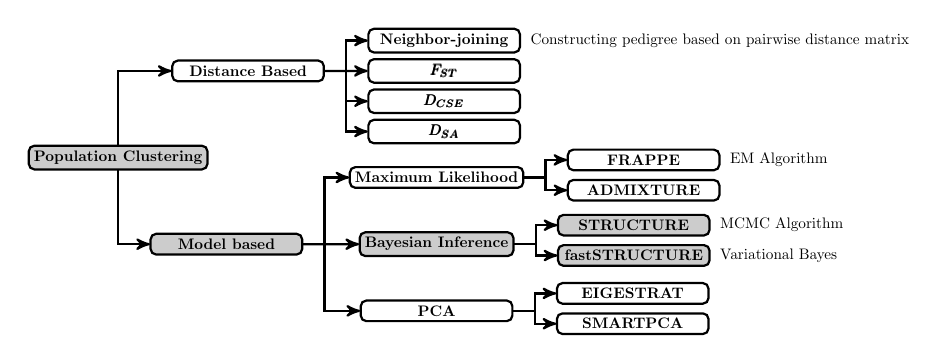
\begin{tikzpicture}[->, >=stealth', auto, node distance=0.7cm, align=right, thick,
	scale=0.55, transform shape,
	main node/.style={rectangle, rounded corners=2pt, draw, font=\bfseries, minimum width=3.5cm},
	main gray/.style={rectangle, fill=black!20, rounded corners=2pt, draw, font=\bfseries, minimum width=3.5cm},
]
\node [main gray] at (-4cm, 0cm) (root) {Population Clustering};
\node [main node] at (-1cm, 2cm) (DistBase) {Distance Based};
\node [main node]                (F_ST) [right=1cm of DistBase] {\pmb{$F_{ST}$}};
\node [main node]                (D_CSE) [below of=F_ST] {\pmb{$D_{CSE}$}};
\node [main node]                (D_SA) [below of=D_CSE] {\pmb{$D_{SA}$}};
\node [main node]                (Neighbor) [above of=F_ST] {Neighbor-joining};
\node () [right=0.1cm of Neighbor] {Constructing pedigree based on pairwise distance matrix};
\node [main gray] at (-1.5cm, -2cm) (ModelBase) {Model based};
\node [main gray]                (Post) [right=1.3cm of ModelBase] {Bayesian Inference};
\node [main node]                (MaxLike) [above=1cm of Post] {Maximum Likelihood};
\node [main node]                (FRAPPE) [above right=-0.1cm and 1cm of MaxLike] {FRAPPE};
\node () [right=0.1cm of FRAPPE] {EM Algorithm};
\node [main node]                (ADMIXTURE) [below of=FRAPPE] {ADMIXTURE};
\node [main gray]                (STRUCTURE) [above right=-0.1cm and 1cm of Post] {STRUCTURE};
\node () [right=0.1cm of STRUCTURE] {MCMC Algorithm};
\node [main gray]                (fastSTRUCTURE) [below of=STRUCTURE] {fastSTRUCTURE};
\node [main node]                (PCA) [below=1cm of Post] {PCA};
\node [main node]                (EIGESTRAT) [above right=-0.1cm and 1cm of PCA] {EIGESTRAT};
\node [main node]                (SMARTPCA) [below of=EIGESTRAT] {SMARTPCA};
%
\draw [->] (root)     |- (DistBase);
\draw [->] (DistBase.east) --++ (0.5, 0) |- (Neighbor);
\draw [->] (DistBase) -- (F_ST);
\draw [->] (DistBase.east) --++ (0.5, 0) |- (D_CSE);
\draw [->] (DistBase.east) --++ (0.5, 0) |- (D_SA);
\draw [->] (root)      |- (ModelBase);
\draw [->] (ModelBase.east) --++ (0.5, 0) |- (MaxLike);
\draw [->] (MaxLike.east) --++ (0.5, 0) |- (FRAPPE);
\draw [->] (MaxLike.east) --++ (0.5, 0) |- (ADMIXTURE);
\draw [->] (ModelBase.east) -- (Post);
\draw [->] (Post.east) --++ (0.5, 0) |- (STRUCTURE);
\draw [->] (Post.east) --++ (0.5, 0) |- (fastSTRUCTURE);
\node () [right=0.1cm of fastSTRUCTURE] {Variational Bayes};
\draw [->] (ModelBase.east) --++ (0.5, 0) |- (PCA);
\draw [->] (PCA.east) --++ (0.5, 0) |- (EIGESTRAT);
\draw [->] (PCA.east) --++ (0.5, 0) |- (SMARTPCA);
\end{tikzpicture}
\end{figure}
\end{frame}

%%%%%%%%%%%%%%%%%%%%%%%%%%%%%%%%%%%%%%%%
\begin{frame}
\frametitle{Association Mapping Methods}
\begin{figure}
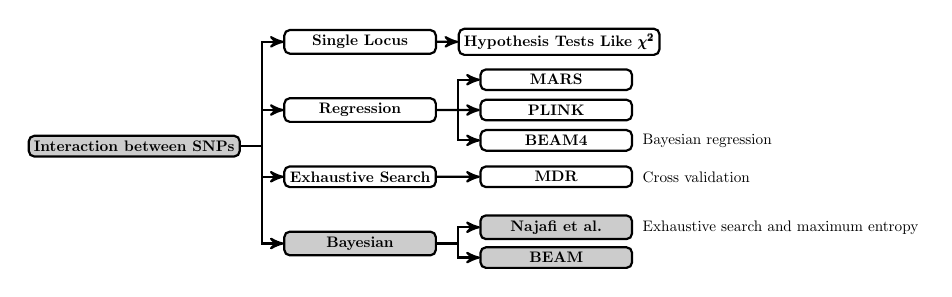
\begin{tikzpicture}[->, >=stealth', auto, node distance=0.7cm, align=center,
	thick, scale=0.55, transform shape,
	main node/.style={rectangle, rounded corners=2pt, draw, font=\bfseries, minimum width=3.5cm},
	main gray/.style={rectangle, fill=black!20, rounded corners=2pt, draw, font=\bfseries, minimum width=3.5cm},
]
\node [main gray] at (4cm, 0cm) (root) {Interaction between SNPs};
\node [main node] (Exh) [below right=0.2cm and 1cm of root] {Exhaustive Search};
\node [main node] (MDR) [right=1cm of Exh] {MDR};
\node () [right=0.1cm of MDR] {Cross validation};
\node [main node] (Reg) [above=1cm of Exh] {Regression};
\node [main node] (PLINK) [right=1cm of Reg] {PLINK};
\node [main node] (MARS) [above of=PLINK] {MARS};
\node [main node] (BEAM4) [below of=PLINK] {BEAM4};
\node () [right=0.1cm of BEAM4] {Bayesian regression};
\node [main node] (Sing) [above=1cm of Reg] {Single Locus};
\node [main node] (Chi2) [right=0.5cm of Sing] {Hypothesis Tests Like \pmb{$\chi^2$}};
\node [main gray] (Bayes) [below=1cm of Exh] {Bayesian};
\node [main gray] (Najafi) [above right=-0.2cm and 1cm of Bayes] {Najafi et al.};
\node () [right=0.1cm of Najafi] {Exhaustive search and maximum entropy};
\node [main gray] (BEAM) [below of=Najafi] {BEAM};
%
\draw [->] (root.east) --++ (0.5, 0) |- (Sing);
\draw [->] (Sing) -- (Chi2);
\draw [->] (Exh) -- (MDR);
\draw [->] (root.east) --++ (0.5, 0) |- (Reg);
\draw [->] (Reg) -- (PLINK);
\draw [->] (Reg.east) --++ (0.5, 0) |- (MARS);
\draw [->] (Reg.east) --++ (0.5, 0) |- (BEAM4);
\draw [->] (root.east) --++ (0.5, 0) |- (Exh);
\draw [->] (root.east) --++ (0.5, 0) |- (Bayes);
\draw [->] (Bayes.east) --++ (0.5, 0) |- (Najafi);
\draw [->] (Bayes.east) --++ (0.5, 0) |- (BEAM);
\end{tikzpicture}
\end{figure}
\end{frame}



%%%%%%%%%%%%%%%%%%%%%%%%%%%%%%%%%%%%%%%%%%%%%%%%%%%%%%%%%%%%%%%%%%%%%%%%%%%%%%%%
\section{Motivation \& Contributions}
\begin{frame}
\frametitle{Motivation \& Contributions}
\begin{enumerate}
\item Unification of pre-processing stage and analysis stages \pause
\item Improving Najafi et al. performance
	\begin{itemize}
	\item Exhaustive search replacement
	\item Reducing false-positive reports
	\end{itemize} \pause
\item Adding population structure to BEAM model
	\begin{itemize}
	\item Better association mapping
	\end{itemize}
\end{enumerate}
\end{frame}



%%%%%%%%%%%%%%%%%%%%%%%%%%%%%%%%%%%%%%%%%%%%%%%%%%%%%%%%%%%%%%%%%%%%%%%%%%%%%%%%
\section{The Proposed Model}
\begin{frame}
\frametitle{Inputs}
\begin{itemize}
\item Bi-allelic samples $X$ from $L$ loci of $N$ individuals
\item Binary disease status, $Y$
\item Number of clusters, $K$
\end{itemize}
%
\begin{figure}[!ht]
\centering
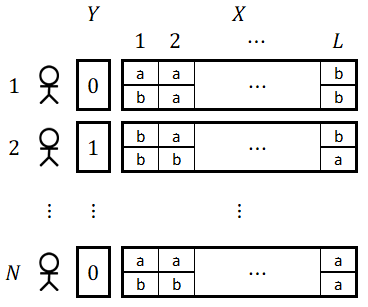
\includegraphics[height=4.2cm]{imgs/Inputs}
\end{figure}
\end{frame}

%%%%%%%%%%%%%%%%%%%%%%%%%%%%%%%%%%%%%%%%
\begin{frame}
\frametitle{Parameters}
\framesubtitle{Individual Parameters}
\begin{itemize}
\item Sub-population of origin of individuals, $Q$
\item Sub-population of origin of alleles, $Z$
\end{itemize}
%
\begin{figure}[!ht]
\centering
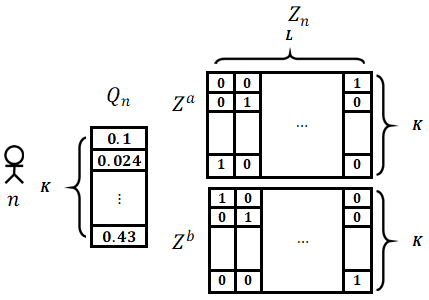
\includegraphics[height=4.2cm]{imgs/IndivParams}
\end{figure}
\end{frame}

%%%%%%%%%%%%%%%%%%%%%%%%%%%%%%%%%%%%%%%%
\begin{frame}
\frametitle{Parameters}
\framesubtitle{Cluster Parameters}
\begin{itemize}
\item Allele frequencies, $P_k$
\item Disease model, $M_k$
	\begin{itemize}
	\item Association status, $I_k$
	\item Disease graph, $G_k = (C_k, \Delta_k)$
	\end{itemize}
\end{itemize}
%
\begin{figure}[!ht]
\centering
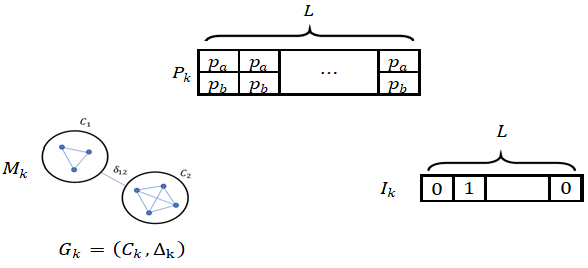
\includegraphics[height=4.2cm]{imgs/ClusterParams}
\end{figure}
\end{frame}

%%%%%%%%%%%%%%%%%%%%%%%%%%%%%%%%%%%%%%%%
\begin{frame}
\frametitle{Assumptions}
\begin{enumerate}
\item Sub-populations are in HWE \pause
\item Allele frequencies are independent \pause
\item Isolated sub-populations, different evolutionary path-ways \pause
\item Independent disease model
\end{enumerate}
\end{frame}

%%%%%%%%%%%%%%%%%%%%%%%%%%%%%%%%%%%%%%%%
\begin{frame}
\frametitle{Sub-Population Related Parameters}
\begin{block}{Sub-Population Joint Probability}
\begin{align*}
\Prob{X, Q, Z, P} &= \Prob{P} \CProb{Z}{Q} \CProb{X}{Z, P}						\\
	&= \Prob{P}
		\prod_{n=1}^N \CProb{Z_{n,l}}{Q_n}
		\prod_{l=1}^L \CProb{X_{n,l}}{P, Z_{n,l}}
\end{align*}
\end{block}
%
\begin{figure}[!ht]
\centering
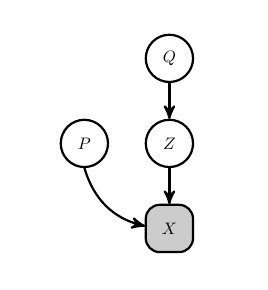
\begin{tikzpicture}[->, >=stealth', auto, node distance=1.8cm, align=right,
	thick, scale=0.6, transform shape,
	param/.style={circle, draw, font=\bfseries, minimum width=1cm},
	obsr/.style={rectangle, rounded corners=5pt, fill=black!20, draw,
				font=\bfseries, minimum width=1cm, minimum height=1cm},
]
\clip (-3, -0.70) rectangle (1.5, 4.25);
\node [obsr]  (X) {$X$};
\node [param] (Z) [above of=X] {$Z$};
\node [param] (P) [left of=Z]  {$P$};
\node [param] (Q) [above of=Z] {$Q$};
%
\draw [->] (P.south) to[bend right=30] (X);
\draw [->] (Z) -- (X);
\draw [->] (Q) -- (Z);
\end{tikzpicture}
\caption{Population structure}
\label{fig:PopStrGraphicalModel}
\end{figure}
\end{frame}

%%%%%%%%%%%%%%%%%%%%%%%%%%%%%%%%%%%%%%%%
\begin{frame}
\frametitle{Association Mapping Related Parameters}
\begin{block}{Disease Model Probability}
\begin{align*}
\CProb{Y_k}{X_k, M_k} & \propto \Prob{Y_k, X_k, M_k}							\\
	& \qquad = \Prob{Y_k, X_k, G_k, I_k}										\\
	& \qquad = \CProb{X_k}{Y_k, G_k, I_k}
		\CProb{G_k}{I_k}
		\Prior{I_k}
		\Prior{Y_k}
\end{align*}
\end{block}
%
\begin{figure}[!ht]
\centering
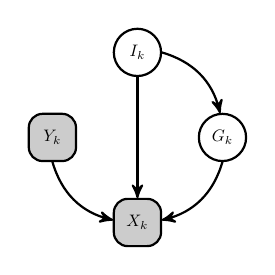
\begin{tikzpicture}[->, >=stealth', auto, node distance=1.8cm, align=right,
	thick, scale=0.6, transform shape,
	param/.style={circle, draw, font=\bfseries, minimum width=1cm},
	obsr/.style={rectangle, rounded corners=5pt, fill=black!20, draw,
				font=\bfseries, minimum width=1cm, minimum height=1cm},
]
\node [obsr]  (X) {$X_k$};
\node  (EPT) [above of=X] {};
\node [param] (I) [above of=EPT] {$I_k$};
\node [obsr]  (Y) [left of=EPT] {$Y_k$};
\node [param] (G) [right of=EPT] {$G_k$};
%
\draw [->] (Y.south) to[bend right=30] (X);
\draw [->] (G.south) to[bend left=30] (X);
\draw [->] (I) -- (X);
\draw [->] (I.east) to[bend left=30] (G);
\end{tikzpicture}
\label{fig:BEAM3GraphicalModel}
\caption{Disease model for $M_k$}
\end{figure}
\end{frame}

%%%%%%%%%%%%%%%%%%%%%%%%%%%%%%%%%%%%%%%%
\begin{frame}
\frametitle{Graphical Model}
\begin{columns}
\column{0.67 \textwidth}
\begin{block}{Joint Probability of All Parameters and Inputs}
\begin{align*}
\Pr(X, &Y, P, Z, Q, M) =
	\Prob{P} \prod_{n=1}^{N} \Big(
	\Prob{Q_n}	\\
	& \quad \times \prod_{l=1}^{L} \Big[
		\CProb{Z_{nl}}{Q_n} \CProb{X_n}{P, Z_{nl}}
	\Big]
\nonumber \\
		& \quad \times \CProb{M_k}{Q_n} \CProb{Y_n}{X_n, M_k}
	\Big).
\label{eq:GenerativeModelProbability}
\end{align*}
\end{block}
\hfill %
\column{0.23 \textwidth}
\begin{figure}[!ht]
\centering
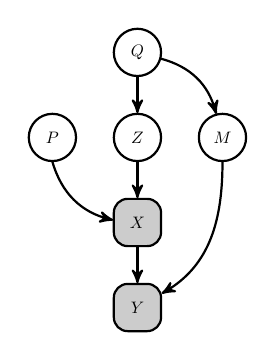
\begin{tikzpicture}[->, >=stealth', auto, node distance=1.8cm, align=right,
	thick, scale=0.6, transform shape,
	param/.style={circle, draw, font=\bfseries, minimum width=1cm},
	obsr/.style={rectangle, rounded corners=5pt, fill=black!20, draw, font=\bfseries, minimum width=1cm, minimum height=1cm},
]
\node [obsr]  (X) {$X$};
\node [obsr]  (Y) [below of=X] {$Y$};
\node [param] (Z) [above of=X] {$Z$};
\node [param] (P) [left of=Z]  {$P$};
\node [param] (Q) [above of=Z] {$Q$};
\node [param] (M) [right of=Z] {$M$};
%
\draw [->] (P.south) to[bend right=30] (X);
\draw [->] (Z) -- (X);
\draw [->] (Q) -- (Z);
\draw [->] (M) to[out=270, in=30] (Y);
\draw [->] (X) -- (Y);
\draw [->] (Q) to[bend left=30] (M);
\end{tikzpicture}
\caption{Complete model}
\label{fig:GenerativeGraphicalModel}
\end{figure}
\end{columns}
\end{frame}

%%%%%%%%%%%%%%%%%%%%%%%%%%%%%%%%%%%%%%%%
\begin{frame}
\frametitle{Priors}
\begin{block}{Priors for sub-populations}
\begin{gather*}
\scalebox{0.75}{$\Prob{Z_{n,l} = k} = \frac{1}{K}$}												\\
\scalebox{0.75}{$\Prob{P_{k,l,\bullet}} = \BetaDist{\beta_1}{\beta_2}, \beta_1 = \beta_2 = 1$}	\\
\scalebox{0.75}{$\Prob{Q_n} = \Dir{\alpha_1, \dots, \alpha_K}, \alpha_i = 1$}
\end{gather*}
\end{block}
\begin{block}{Priors for association mapping}
\begin{gather*}
\scalebox{0.75}{$\Prob{Y_{n} = 1} = 1 - \Prob{Y_{n} = 0} = 0.01$}								\\
\scalebox{0.75}{$\Prob{I_{k,l} = 1} = 1 - \Prob{I_{k,l} = 0} = 0.01$}							\\
\scalebox{0.75}{$\Prob{\delta_{i,j} = 1} = 1 - \Prob{\delta_{i,j} = 0} = 0.01$}					\\
\text{Pitman-Yor Process} \begin{cases}
	\text{old clique} & \scalebox{0.75}{$\CProb{x_l \in c_i}{C_k,I} = \frac{n_k - \beta}{i + \alpha}$}					\\
	\text{new clique} & \scalebox{0.75}{$\CProb{x_l \in c_{W + 1}}{C_k,I} = \frac{\alpha + W \beta}{i + \alpha}$}
\end{cases}
\end{gather*}
\end{block}
\end{frame}



%%%%%%%%%%%%%%%%%%%%%%%%%%%%%%%%%%%%%%%%%%%%%%%%%%%%%%%%%%%%%%%%%%%%%%%%%%%%%%%%
\section{Inference}
\begin{frame}
\frametitle{Complete Inference of Parameters}
\begin{algorithm}[H]
\small
%\onehalfspacing
\caption{Inference of parameters}
\label{alg:ParametersInference}
\begin{algorithmic}
%%%%%%%%%%%%%%%%%%%%%%%%%%%%%%%%%%%%%%%%%%%%%%%%%%
\State Initialize $P^{(0)} \sim \Prior{P}$,
	$Q^{(0)} \sim \Prior{Q}$,
	and $Z \sim \CProb{Z}{Q}$.
\For { $k = 1:K$ }
	\State Initialize $I_k^{(0)} \sim \Prior{I_k}$.
	\State Partition SNPs by Pitman-Your process into $C_k^{(0)}$.
	\State Initialize $G_k^{(0)} = \left( C_k^{(0)}, \Delta_k^{(0)} \right) \sim \CProb{G_k}{I_k}$.
\EndFor
%%%%%%%%%%%%%%%%%%%%%%%%%%%%%%%%%%%%%%%%%%%%%%%%%%
%%%%%%%%%%%%%%%%%%%%%%%%%%%%%%%%%%%%%%%%%%%%%%%%%%
\For{ $r = 1:MaxIterations$ }
%%%%%%%%%%%%%%%%%%%%%%%%%%%%%%%%%%%%%%%%%%%%%%%%%%
	\State Update parameters $Z^{(r)}$, $Q^{(r)}$, and $P^{(r)}$.
%%%%%%%%%%%%%%%%%%%%%%%%%%%%%%%%%%%%%%%%%%%%%%%%%%
	\State Pick an unassociated SNP $x_i$, change its membership with $\Prob{I_{ki} = 1}$.
%%%%%%%%%%%%%%%%%%%%%%%%%%%%%%%%%%%%%%%%%%%%%%%%%%
	\State Calculate $\gamma = \frac{\Prob{x_i + X_{k, 1}, Y, G_k, I_{ki} = 1}}{\Prob{X_{k, 1}, Y, G_k, I_{ki} = 0}}$.
	\State Draw $u \sim \Unif{0}{1}$.
	\If { $u < \gamma$ }
		\State Add $x_i$ to $X_{k, i}$, set $I_{ki} = 1$, and Update $G_k^{(r)}$.
	\EndIf
	\State Randomly select $c_i$ and $c_j$ from $C_K$, merge or exchange SNPs.
%%%%%%%%%%%%%%%%%%%%%%%%%%%%%%%%%%%%%%%%%%%%%%%%%%
\EndFor
\end{algorithmic}
\end{algorithm}
\end{frame}



%%%%%%%%%%%%%%%%%%%%%%%%%%%%%%%%%%%%%%%%%%%%%%%%%%%%%%%%%%%%%%%%%%%%%%%%%%%%%%%%
\section{Synthetic Dataset}
\begin{frame}
\frametitle{Synthetic Dataset}
\begin{enumerate}
\item Simulation
	\begin{itemize}
	\item More accurate in biological terms
	\item Time consuming
	\end{itemize}
\item Generative process
	\begin{itemize}
	\item Simple and fast
	\end{itemize}
\end{enumerate}
\end{frame}

%%%%%%%%%%%%%%%%%%%%%%%%%%%%%%%%%%%%%%%%
\begin{frame}
\frametitle{Dataset generation}
\begin{algorithm}[H]
\caption{Generative process for genotype dataset}
\label{alg:GenotypeGeneration}
\begin{algorithmic}
%%%%%%%%%%%%%%%%%%%%%%%%%%%%%%%%%%%%%%%%%%%%%%%%%%
\State Draw $P_{kl} \sim \BetaDist{\beta_{kla}}{\beta_{klb}}$.
\For{ $n = 1:N$ }
	\State Draw $Q_n = ( Q_{n1}, \cdots, Q_{nK} ) \sim \Dir{\alpha_n}$.
	\For{ $l = 1:L$ and $j \in \{ a, b \}$}
		\State Draw allele origin from $\Prob{Z_{nlj} = k} = Q_{nk}, k = 1, \dots, K$.
		\State Draw genotype from $X_{nl} \sim \CProb{P_{kl}}{Z_{nlj}}$.
	\EndFor
	\State Draw disease model from $M_k \sim \CProb{M}{Q_n}$.
	\State Draw disease status from $\CProb{Y_n}{X_n, M_k}$.
\EndFor
\end{algorithmic}
\end{algorithm}
\end{frame}

%%%%%%%%%%%%%%%%%%%%%%%%%%%%%%%%%%%%%%%%
\begin{frame}
\frametitle{Disease Status Label}
\framesubtitle{Disease Loci}
\begin{table}[!ht]
\caption{Disease Model}
\label{tab:DiseaseModelSNPs}
\centering
%\onehalfspacing
\subfigure[Sub-population 1]{
\begin{tabularx}{0.45\textwidth}{|X|X|}
\hline
\centering \bf{Locus} & \centering \bf{SNP} \tabularnewline
\hline
1724 & 0							\\
2620 & 0							\\
6005 & 1							\\
\hline
\end{tabularx}
}
%%%%%%%%%%%%%%%%%%%%%%%%%%%%%%%%%%%%%%%%%%%%%%%%%%%%%%%%%%%%%%%%%%%%%%%%%%%%%%%
\subfigure[Sub-population 2]{
\begin{tabularx}{0.45\textwidth}{|X|X|}
\hline
\centering \bf{Locus} & \centering \bf{SNP} \tabularnewline
\hline
578 & 1								\\
3786 & 2							\\
9970 & 1							\\
\hline
\end{tabularx}
}
\end{table}
%
\begin{gather}
\operatorname{logit} \left( p_n \right) = 1.5 ( X_{k,n1} \cdot X_{k,n2} \cdot X_{k, n3} ),
\nonumber \\ %%%%%%%%%%%%%%%%%%%%%%%%%%%%%%%%%%%%%%%%
Y_n \sim \Bernoulli{p_n}
\nonumber
\label{eq:LogitY}
\end{gather}
\end{frame}



%%%%%%%%%%%%%%%%%%%%%%%%%%%%%%%%%%%%%%%%%%%%%%%%%%%%%%%%%%%%%%%%%%%%%%%%%%%%%%%%
\section{Results}
\begin{frame}
\frametitle{Results}
\framesubtitle{Clustering}
Comparison of accuracy of clustering for $K = 2$, for $L = 10000$:
\begin{figure}[!ht]
\centering
\subfigure[$MAF=1\%$]{
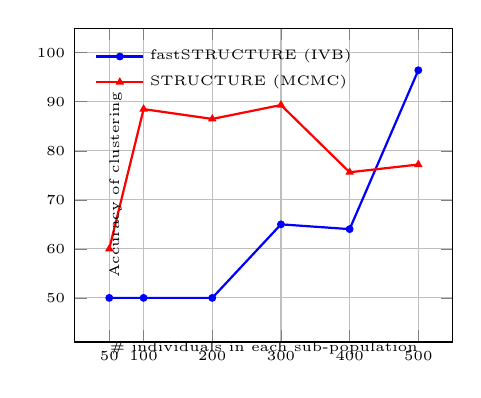
\begin{tikzpicture}
\begin{axis}[
	scale=0.7,
	grid=both,
    label style={font=\tiny},
    ticklabel style={font=\tiny},
    xlabel style={at={(0.5, 0.03)}},
    ylabel style={at={(0.15, 0.5)}},
    xmin=0, xmax=550, ymin=41, ymax=105,
    xtick={50, 100, 200, ..., 500}, ytick={0, 10, ..., 110},
    xlabel=\# individuals in each sub-population,
    ylabel=Accuracy of clustering,
    legend style={font=\tiny,
		fill=none,		% Transparent
		draw=none},		% No border
    legend cell align=left,
    legend pos=north west,
    legend entries={{fastSTRUCTURE (IVB)}, {STRUCTURE (MCMC)}},
]
% fastSTRUCTURE
\addplot[color=blue, mark=*, thick, mark options={scale=0.5}] coordinates {
   (50, 50.0) (100, 50.0) (200, 50.0) (300, 65.0) (400, 64.025) (500, 96.43) };
% STRUCTURE
\addplot[color=red, mark=triangle, thick, mark options={scale=0.5}] coordinates {
    (50, 60) (100, 88.5) (200, 86.5) (300, 89.333) (400, 75.625) (500, 77.2) };
\end{axis}
\end{tikzpicture}
}\hfill
%%%%%%%%%%%%%%%%%%%%%%%%%%%%%%%%%%%%%%%
\subfigure[$MAF=2\%$]{
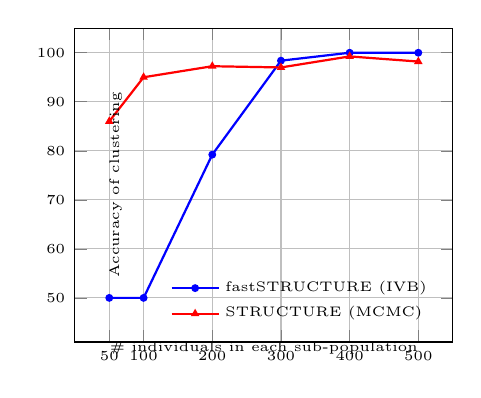
\begin{tikzpicture}
\begin{axis}[
	scale=0.7,
	grid=both,
    label style={font=\tiny},
    ticklabel style={font=\tiny},
    xlabel style={at={(0.5, 0.03)}},
    ylabel style={at={(0.15, 0.5)}},
    xmin=0, xmax=550, ymin=41, ymax=105,
    xtick={50, 100, 200, ..., 500}, ytick={0, 10, ..., 110},
    xlabel=\# individuals in each sub-population,
    ylabel=Accuracy of clustering,
    legend style={font=\tiny,
		fill=none,		% Transparent
		draw=none},		% No border
    legend cell align=left,
    legend pos=south east,
    legend entries={{fastSTRUCTURE (IVB)}, {STRUCTURE (MCMC)}},
]
% fastSTRUCTURE
\addplot[color=blue, mark=*, thick, mark options={scale=0.5}] coordinates {
   (50, 50.0) (100, 50.0) (200, 79.225) (300, 98.383) (400, 100.0) (500, 100.0) };
% STRUCTURE
\addplot[color=red, mark=triangle, thick, mark options={scale=0.5}] coordinates {
    (50, 86) (100, 95) (200, 97.25) (300, 97) (400, 99.25) (500, 98.2) };
\end{axis}
\end{tikzpicture}
}
\label{fig:ClusteringK2}
\end{figure}
\end{frame}

%%%%%%%%%%%%%%%%%%%%%%%%%%%%%%%%%%%%%%%%
\begin{frame}
\frametitle{Results}
\framesubtitle{Association Mapping}
Posterior of associated SNPs for StrBEAM and BEAM3\\
$N=1000$, $L=10000$, $K=2$, and $\text{MAF}=5\%$
\begin{figure}[!ht]
\centering
\subfigure[StrBEAM] { 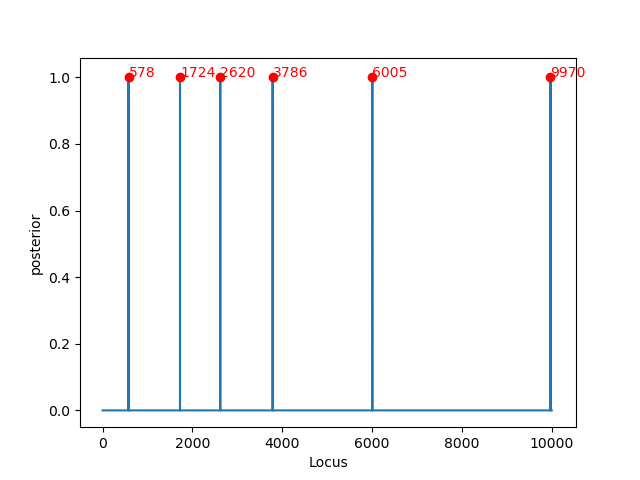
\includegraphics[height=4.2cm]{imgs/MyAlg-posterior-test14} }
\subfigure[BEAM3]	{ 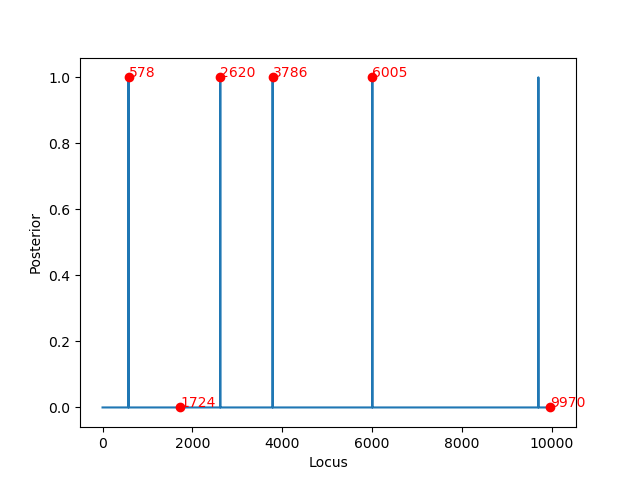
\includegraphics[height=4.2cm]{imgs/beam3-posterior-test14} }
\label{fig:ThreeWayNoCluster}
\end{figure}
\end{frame}



%%%%%%%%%%%%%%%%%%%%%%%%%%%%%%%%%%%%%%%%%%%%%%%%%%%%%%%%%%%%%%%%%%%%%%%%%%%%%%%%
\section{Future Works}
\begin{frame}
\frametitle{Future Works}
\begin{itemize}
\item More complex synthetic datasets
	\begin{itemize}
	\item Admixture populations
	\item More disease associated scenarios
	\end{itemize} \pause
\item Development of model
	\begin{itemize}
	\item Non-case-control datasets like QTL (Quantitative Trait Locus)
	\item Gene Expression
	\end{itemize} \pause
\item Real datasets
	\begin{itemize}
	\item WTCCC (Wellcome Trust Case Control Consortium)
	\item Other model organisms, like mouse
	\end{itemize}
\end{itemize}
\end{frame}



%%%%%%%%%%%%%%%%%%%%%%%%%%%%%%%%%%%%%%%%%%%%%%%%%%%%%%%%%%%%%%%%%%%%%%%%%%%%%%%%
\section{References}
\begin{frame}
\frametitle{References and Source Code}
Main References:
\pagestyle{empty}
{
\tiny
\begin{thebibliography}{99}
\baselineskip12pt
\bibitem[Najafi {\it et al.} (2019)]{Najafi:et:al:2019} Najafi A., Janghorbani S., Motahari S. A., and Fatemizadeh E. (2019), Statistical Association Mapping of Population-Structured Genetic Data, {\it IEEE/ACM Transactions on Computational Biology and Bioinformatics,} {\bf 16}, 638-649.
\bibitem[Pritchard {\it et al.} (2000)]{Pritchard:et:al:2000} Pritchard J.  K., Stephens M., and Donnelly P. (2000), Inference of Population Structure Using Multilocus Genotype Data, {\it Genetics Society of America,} {\bf 155}, 945-959.
\bibitem[Raj {\it et al.} (2014)]{Raj:et:al:2014} Raj A., Stephens M., Pritchard J. K. (2014), fastSTRUCTURE: Variational Inference of Population Structure in Large SNP Data Sets, {\it Genetics,} {\bf 197}, 573-589.
\bibitem[Zhang (2012)]{Zhang:2012} Zhang Y. (2012), A Novel Bayesian Graphical Model for Genome-Wide Multi-SNP Association Mapping, {\it Genomic Epidemiology,} {\bf 36}, 36-47.
\newline
\newline
\newline
\end{thebibliography}
}
Source code is available at:
\Href{https://github.com/VahidHeidari/StrBEAM}
\end{frame}



%%%%%%%%%%%%%%%%%%%%%%%%%%%%%%%%%%%%%%%%%%%%%%%%%%%%%%%%%%%%%%%%%%%%%%%%%%%%%%%%
\section*{Contacts}
\begin{frame}
\frametitle{Contacts}
\begin{table}[H]
\begin{tabularx}{0.6\linewidth}{l>{\raggedright\arraybackslash}X}

\includegraphics[height=2cm]{imgs/VHeidari}
&
\parbox[b][1.5cm]{25mm}{
Vahid Heidari:\newline
\Href{vahid.heidari@ut.ac.ir}
}
\\

\includegraphics[height=2cm]{imgs/MAmini}
&
\parbox[b][1.5cm]{30mm}{
Morteza Amini:\newline
\Href{morteza.amini@ut.ac.ir}
}
\\
\raisebox{-0.9cm}{
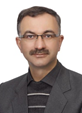
\includegraphics[height=2cm]{imgs/MTaheri}
}
&
Seyed Mahmoud Taheri:\newline
\Href{sm\_taheri@ut.ac.ir}
\\
\end{tabularx}
\end{table}
\end{frame}

%%%%%%%%%%%%%%%%%%%%%%%%%%%%%%%%%%%%%%%%
\begin{frame}
\center{Thank you}
\begin{figure}[!ht]
\centering

\includegraphics[width=13cm]{imgs/Questions}
\end{figure}
\end{frame}

\end{document}

